\documentclass[10pt,letterpaper]{article}
\usepackage[utf8]{inputenc}
\usepackage{amsmath}
\usepackage{amsfonts}
\usepackage{amssymb}
\usepackage{graphicx}
\usepackage{url}
\usepackage{wrapfig}
\usepackage{footbib}
\author{Christopher C. Lamb}
\begin{document}

\begin{wrapfigure}{r}{.5\textwidth}
\begin{center}
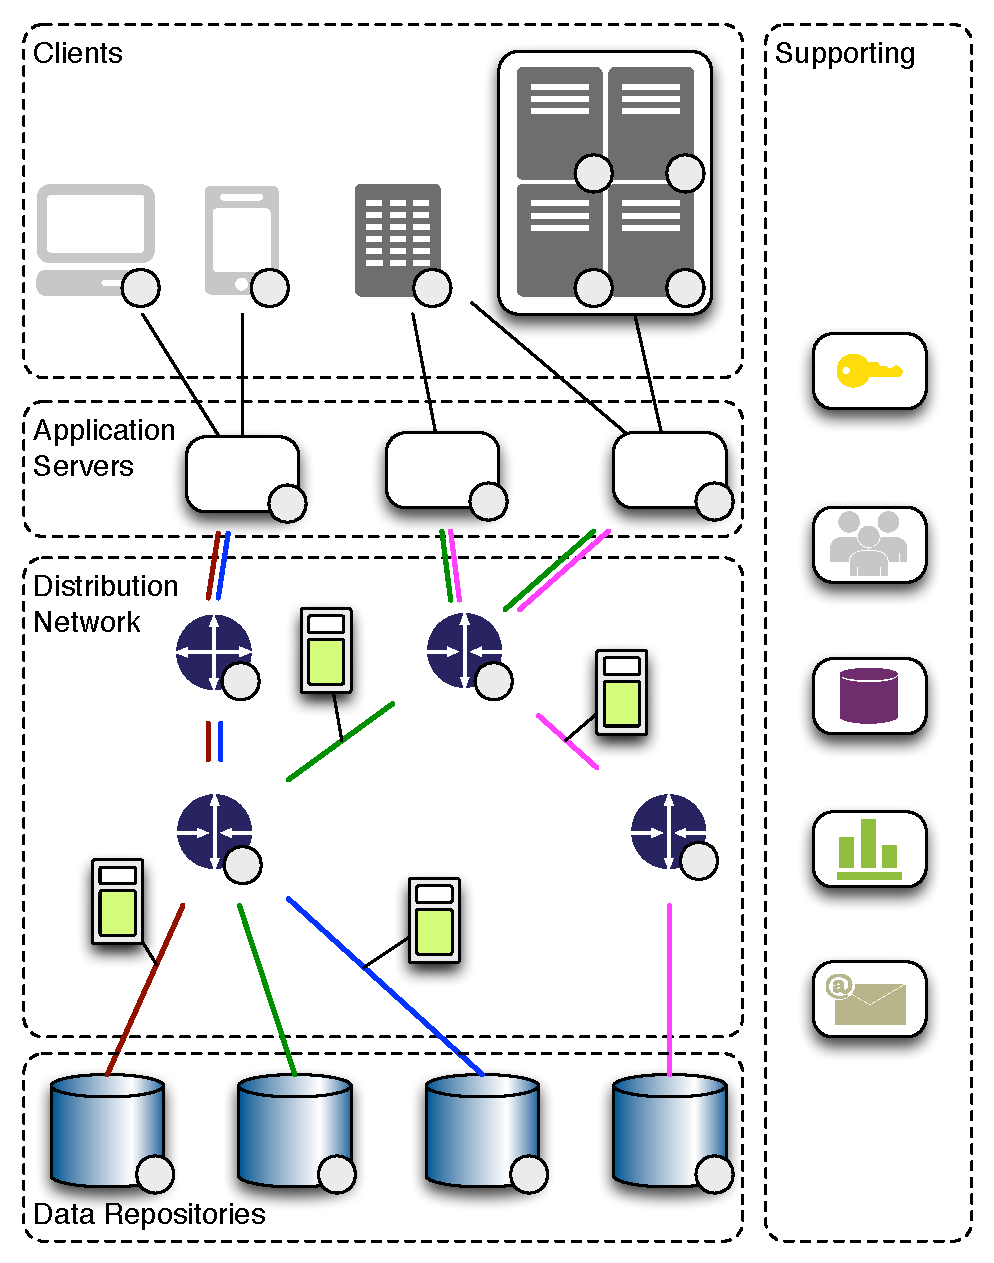
\includegraphics[width=.47\textwidth]{./images/network.pdf}
\end{center}
\caption{A notional view of the Nublu system, showing various required and provided services in an end-to-end perspective.}
\label{fig:network}
\end{wrapfigure}

\paragraph{Threat Model} In order to understand the security controls needed for Nublu infrastructure, we first need to understand the threat landscape.  Today, the Cloud Security Alliance~\footcite{csa} maintains an up-to-date list of the most active security threats to cloud systems.  The most recent version, for 2013, outlines the nine most common security threats that exist today as well as security controls that can help alleviate the risk imposed by those threats~\footcite{csa-noni:13}.  Out threat model is based on this list of current cloud threats.  

%We will extract salient controls from this model, and build them into developed infrastructure if possible.  If not, we will outline specifically how those controls could be integrated, or why they are not applicable.

Figure \ref{fig:network} shows a notional representation of our proposed Nublu system.  This shows the primary catagories of services we will provision, as well as supporting services.  To begin with, at the bottom of the figure, we have a collection of {\sl Data Repositories}.  These repositories can be of a variety of types, ranging from graph databases(like Neo4j~\footcite{neo4j}) to document databases (like MongoDB~\footcite{mongodb}) to data structure databases (like Redis~\footcite{redis}) to relational databases. These data repositories exchange information via a {\sl Distribution Network}.  This distribution network transfers information at a variety of security and quality-of-service (QoS) levels, based on the content traversing the network.  This figure shows {\sl Secure Data Objects} traversing the distribution network over links provisioned at varying security and QoS levels.  The individual network links are managed and connected by control nodes, similar to switches or routers, that manage the flow of information and data transmission performance through the distribution network.  The system delivers information to {\sl Application Servers} that deliver information to {\sl Clients}.  All elements have embedded information usage and distribution management components, and depend on common services to provide and enforce security controls.  Specific common services from top to bottom include key management and public key infrastructure (PKI), identity and access control (ICAM), directory, monitoring and management, and messaging.  Within this view, the Nublu system is responsible for the technical performance of services within the Repository, Distribution Network, and Application Server layers.

This system will provision infrastructure on demand at various levels of service and security via software defined infrastructure and network management. These levels can then dynamically change based on the environment, increasing performance or security based on external events and risk.

\paragraph{Data Breaches} Data breaches are the most common issue facing cloud deployed information today.  Misconfigured databases or multi-tenant virtualization platforms can expose sensitive data to theft.  Recent research highlights these issues, demonstrating how attackers can exploit side-channel weaknesses to steal sensitive information ~\footcite{ZhJuReRi:12}.  Other recent breaches demonstrate how poor governance and data retention practices can lead to the leak of large swaths of sensitive information as well~\footcite{De:12}.  Data breaches differ from data loss as breaches imply a leakage of data to unauthorized personnel, while data loss implies permanent loss of information.  Ergo, breaches impact all levels of concern within the Nublu system, ranging from repositories through the distribution network to application servers. 

%Data backup and retention policies are outside the scope of our work and should be handled by the underlying infrastructure managers.  We do however need to provide guidance for how to support controls that have specific system impact on Nublu.  The specific controls identified to address this threat include:

\paragraph{Data Loss} Data loss is tied to the permanent loss of information via deletion, hardware destruction, or other permanent means. This threat applies to individuals storing information in various cloud services as well as organizations and information stored in systems owned and on premises or managed by third parties. In either case, the data loss can be the result of malicious actors or natural events.  Whatever the cause organizations must be prepared to reconstitute lost information. In our system, data loss threats primarily impact the data repository layer. Any data stored in any repositories must support efficient, effective, and secure backup to avoid this threat.

\paragraph{Hijacking} Service and account hijacking are still relevant threats, and such credentials are, by definition, the primary target of phishing attempts.  As such, they need to be actively protected, not shared, and two-factor identification should be utilized whenever possible.  Though specific ICAM services are outside the scope of this work, developed system must support interfaces to such systems.  Furthermore, PKI and other key management systems must be strongly secured to protect against unauthorized key leakage and associated system damage.  Overall, this threat has wide impact on Nublu.  It affects each layer, and all system agents.  System agents must be authenticated and be authorized to act within the system.  Usage management components are extensions of the ICAM system and make decisions regarding data distribution and must also be secured and authenticated.  All credentials associated with these components must be protected from exfiltration or unauthorized access, and must be able to be quickly suspended in case of compromise.

\paragraph{Interfaces} Interfaces to cloud systems must also be secured.  Not only can malicious actors gain access to cloud-stored information and services via service hijacking, they can also compromise these services via exploing insecure programming interfaces (APIs).  All major commercial cloud service providers support programmatic access to their platforms~\footcite{rackspace-api:13,amazon-api:13}, and Nublu will be no exception from that trend.  In fact, the integration of security controls into the cloud framework and extensive use of software defined infrastructure and networks will increase Nublu's susceptibility to this particular threat.  This threat impacts all service layers and supporting services, as they are all software systems consuming and providing interfaces for external access.

\paragraph{Denial of Service} Denial of service attacks are common and expected within large scale, visible systems.  Government and military systems must be designed to handle large scale denial of service attacks as they are guaranteed when engaged with a hostile power in any way.  In fact, denial of service attacks are commonplace today and typically used by extra-national political organizations and criminal gangs toward a variety of ends, ranging from extortion to simple bragging rights.  Though all components of Nublu are susceptible to Denial of Service attacks, some specific parts of Nublu are more vulnerable than others.  Specific common services, for example, like monitoring and management can be exploited to bring the system down.  ICAM and PKI systems can be used to bring down the system as well if not appropriately hardened.

\paragraph{Insider Threat} Insider threat issues are notoriously difficult for organizations to protect themselves from.  Generally, staff vetting and background checks are primary methods through which organizations try to address insider threat, with some success, though there have been well publicized failures over the past few years with this approach.  Monitoring and usage data collection, as well as observing the principle of least privilege, are common contributors to lessening the risk of insider threat.  Specific insider threat protections are outside of the scope of Nublu, but some of the associated monitoring and management systems can very well be used to contribute to insider threat detection.  Supporting robust authentication and authorization capabilities is also paramount.

\paragraph{Service Abuse} Cloud systems can be compromised and used toward unauthorized ends.  For example, virtual machines (VMs) running within a cloud environment can be used by malicious actors to store malware, stolen digital property, or to attack stolen encrypted information~\footcite{ZhJuReRi:12}.  Nublu is vulnerable to this kind of abuse in all three service layers.  Data storage can be abused to save illicit information, just as virtualized application servers can be compromised for computational horsepower or as pivot points for distributed denial of service attacks.  Likewise, networks can be compromised to transfer stolen digital goods or to hide unauthorized communication.

\paragraph{Due Diligence} Due diligence addresses the need for organizations to adopt cloud computing systems with a clear understanding of the implications of this kind of technology.  Organizations will frequently migrate operations into cloud environments without organizational expertise in the technology or management issues that will arise, leading to mistakes that could have been avoided.  This is primarily a management issue with little impact on Nublu.

\paragraph{Shared Technology} Multi-tenant systems introduce new vulnerabilities into distributed computing systems.  Whether the vulnerabilities enable tenant-to-tenant attacks or tenant-to-infrastructure attacks, Nublu is very vulnerable to thse kinds of threats.  Nublu is heavily virtualized --- hosts are virtualized, networks are virtualized, and data repositories are virtualized to maximize flexibility and efficiency.

\paragraph{Impact on Nublu}
The majority of these threats impact Nublu work and need to be handled by security controls designed into the system rather than controls injected into Nublu as an afterthought.  The only control that does not apply to the Nublu system is {\sl Due Diligence}, in the context of the definition supplied by the CSA~\footcite{csa-noni:13}.  We will then categorize other threats by actual risk, as opposed to perceived risk, and then by alleviating security controls, deliberately not addressing threats that have controls that are outside of the scope of Nublu.

This cursory analysis trims the list of critical threats from eight to four.  First, both {\sl Data Loss} and {\sl Service Abuse} are rectified via controls that are outside toe scope of Nublu.  Potential data loss is alleviated via data retention and risk policies, environment assessments, and equipment location, all of which are tied to specific production environments the analysis of which are outside of the scope of Nublu work.  Service abuse controls include legal preparation and acceptable use policies, again areas outside of Nublu scope.  Lower priority items, threats with lower actual risk, include {\sl Insider Threat} and {\sl Shared Technology}.  These will be lower priority threats for the team to address.

This leaves a group of four priority threats we must address within Nublu, including {\sl Data Breaches}, {\sl Hijacking}, {\sl Interfaces}, and {\sl Denial of Service}.  Looking over these threats, we have a list of baseline controls defined by the CSA~\footcite{csa-ccmv3:13} that apply to Nublu:

\begin{itemize}
\item {\bf CCM DG-04:} {\sl Data Governance --- Retention Policy}
\item {\bf CCM DG-05:} {\sl Data Governance --- Secure Disposal}
\item {\bf CCM DG-06:} {\sl Data Governance --- Non-Production Data}
\item {\bf CCM DG-07:} {\sl Data Governance --- Information Leakage}
\item {\bf CCM DG-08:} {\sl Data Governance --- Risk Assessments}
\item {\bf CCM IS-04:} {\sl Information Security --- Baseline Requirements}
\item {\bf CCM IS-07:} {\sl Information Security --- User Access Policy}
\item {\bf CCM IS-08:} {\sl Information Security --- User Access Restriction/Authorization}
\item {\bf CCM IS-09:} {\sl Information Security --- User Access Revocation}
\item {\bf CCM IS-10:} {\sl Information Security --- User Access Reviews}
\item {\bf CCM IS-18:} {\sl Information Security --- Encryption}
\item {\bf CCM IS-19:} {\sl Information Security --- Encryption Key Management}
\item {\bf CCM IS-22:} {\sl Information Security --- Incident Management}
\item {\bf CCM OP-03:} {\sl Operations Management --- Capacity/Resource Planning}
\item {\bf CCM RS-07:} {\sl Resiliency --- Equipment Power Failures}
\item {\bf CCM SA-02:} {\sl Security Architecture --- User ID Credentials}
\item {\bf CCM SA-03:} {\sl Security Architecture --- Data Security/Integrity}
\item {\bf CCM SA-04:} {\sl Security Architecture --- Application Security}
\item {\bf CCM SA-06:} {\sl Security Architecture --- Production/Non-Production Environments}
\item {\bf CCM SA-07:} {\sl Security Architecture --- Remote User Multi-Factor Authentication}
\item {\bf CCM SA-14:} {\sl Security Architecture --- Audit Logging / Intrusion Detection}
\end{itemize}

Note that this is not a list of all controls and approaches that must be used to provide assured information sharing.  Rather, this is a list of controls that must be in place or supported to provide a competent security baseline from which we can begin Nublu development.  Note, not all controls in this list are within the scope of Nublu work.  While that may be the case, the Nublu system must identify the interfaces and support those external controls require, and implement those interfaces and whatever support is needed to facilitate external control integration.  Controls that are within Nublu scope must be implemented at a technology readiness level commensurate with the Nublu project as a whole.

\footbibliography{bib/tm}
\footbibliographystyle{plain}

\end{document}